Implementado los diseños, para probar el perfilador se utilizó el haz de un láser HeNe a la salida de una fibra óptica con colimador Thorlabs F220FC-A

\subsection{Mediciones preliminares con el perfilador}
Los primeros prototipos del perfiladori, en el marco de Laboratorio 6, se utilizaron para medir el haz de un laser HeNe a la salida de una fibra óptica Thorlabs F220FC-A\cite{thorlabs_fc}, con un tamaño del haz en plano focal nominal de 2$\,$mm en ambos ejes y una divergencia de 0.020$^\circ$. Se hicieron mediciones manuales de este haz para constrastar y calibrar el perfilador.

Los datos medidos están en la figura \ref{fig:perfilador/calibracion_preliminar}, donde el error de la intensidad fue estimado con la variación de la intensidad y el error acusado por el fabricante del instrumental. El error en las abscisas está graficado, pero es despreciable.

\begin{figure}[H]
    \centering
    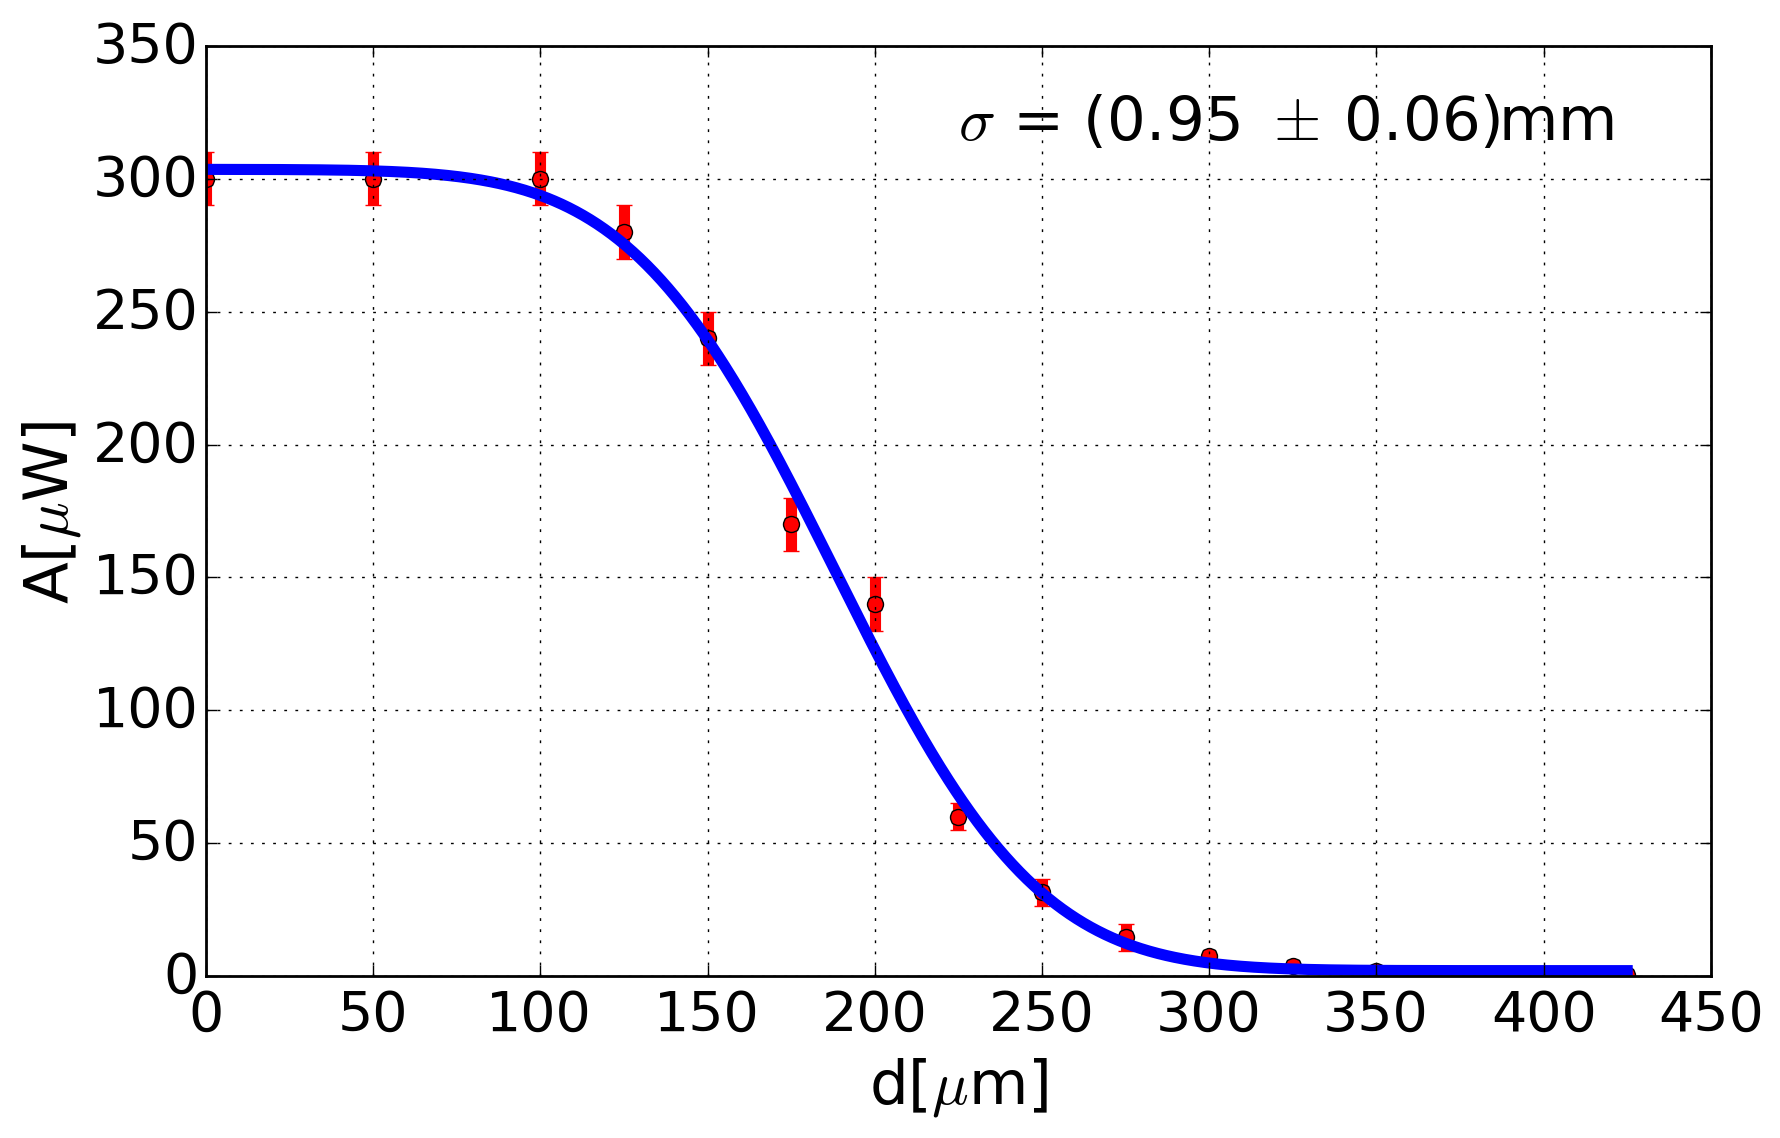
\includegraphics[width=0.55\textwidth]{fig/perfilador/calibracion_preliminar}
    \caption{Perfilación del haz utilizado de forma manual, con el ajuste efectuado. El error en la posición está graficado pero es despreciable}
    \label{fig:perfilador/calibracion_preliminar}
\end{figure}

Podemos ver que esa figura también se agregó el ajuste de la función error. De ese ajuste, el único parámetro que interesa es el ancho medio, que es la mitad del tamaño del haz, ya que la amplitud depende fuertemente del sensor utilizado (y además puede variar, si se usa el fotodiodo, si cambia la resistencia de carga). Tampoco es necesario saber, para las aplicaciones del laboratorio, la intensidad máxima absoluta del haz.

El ajuste efectuado acusa un valor de tamaño medio de $\sigma = (0,95\pm0,06)\,$mm, y recordemos que del colimador utilizado sale un haz con un tamaño de 2$\,$mm en el plano focal, por lo que el valor acusado por el fabricante parece estar bien tabulado. Este valor de $\sigma$ representa la calibración con la que se contrastará el perfilador.

En la figura \ref{fig:perfilador/preliminar_fit} se puede ver los datos obtenidos del microcontrolador.

\begin{minipage}[c]{0.55\textwidth}
\begin{figure}[H]
    \centering
    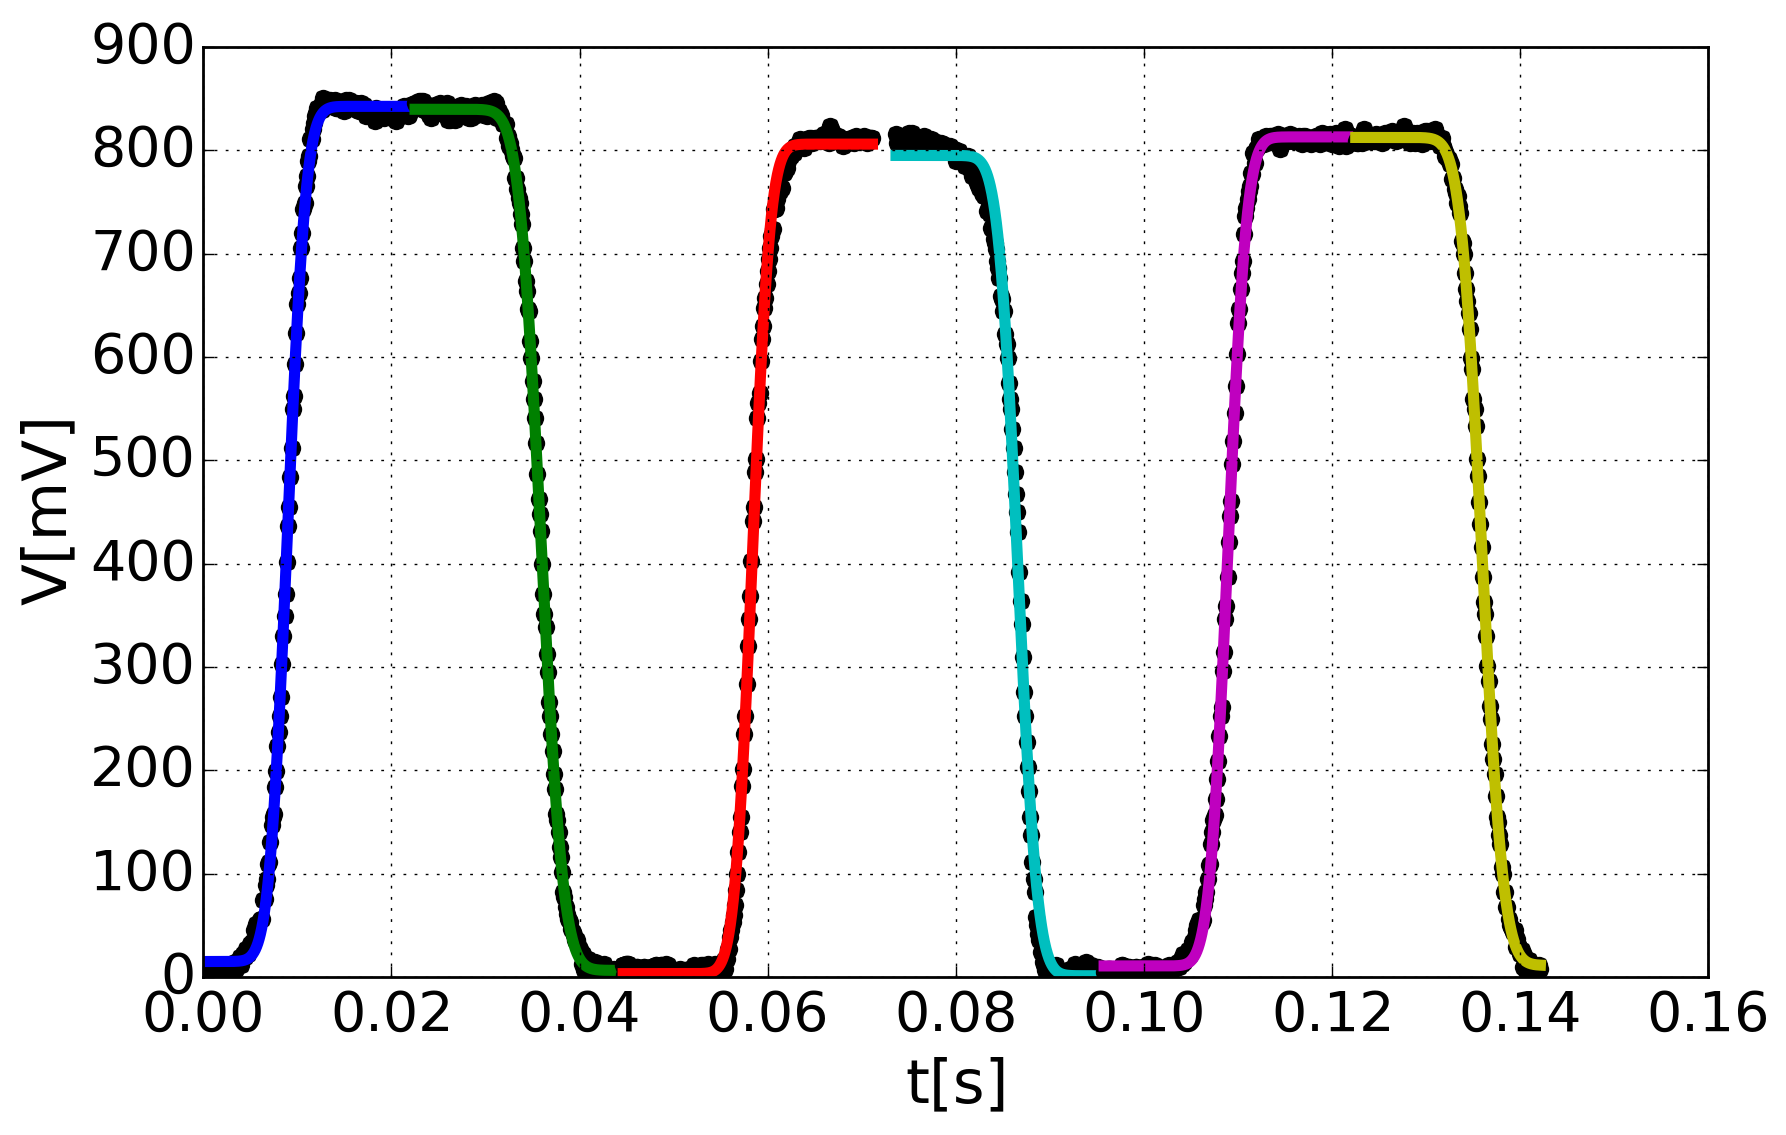
\includegraphics[width=0.8\textwidth]{fig/perfilador/preliminar_fit}
    \caption{Datos medidos con el perfilador a la salida del colimador del SPIM, con las transiciones separadas y ajustadas}
    \label{fig:perfilador/preliminar_fit}
\end{figure}
\end{minipage}
\begin{minipage}[c]{0.35\textwidth}
    \begin{table}[H]
        \centering
        \begin{tabular}{c|c}
            Perfil & $\sigma[\text{mm}]$ \\ \hline
            1 & 1,95 $\pm$ 0,21 \\
            2 & 2,34 $\pm$ 0,24 \\
            3 & 1,88 $\pm$ 0,21 \\
            4 & 2,05 $\pm$ 0,24 \\
            5 & 1,97 $\pm$ 0,21 \\
            6 & 2,27 $\pm$ 0,24 \\
        \end{tabular}
        \caption{}
        \label{tbl:perfilador/preliminar_fit}
    \end{table}
\end{minipage}
\\ \\
Se observa diferencias entre las diferentes transiciones, en especial las que se esperan que sean idénticas (ya que el tambor obtura en el mismo plano el haz para obtenerlas), de hasta 0,2$\,$mm, lo que significa un error de 20\%. No solo eso, se observa una discrepancia del 100\%, es decir un 1$\,$mm, con la calibración (y el tamaño del haz tabulado por el fabricante del colimador). 

Esto lleva a diseñar un tambor metálico, como ya se mencionó, y nuevos diseños del soporte del perfilador.

\subsection{Calibración y mediciones del perfilador}
Habiendo hecho mediciones con los primeros prototipos en Laboratorio 6, se pasó a medir el perfil, en Laboratorio 7, con el tercer y cuarto prototipo (\ref{fig:perfilador/soporte_v3} y \ref{fig:perfilador/soporte_v4}) con el tambor de metal, esta vez a la salida de una colimador de fibra Thorlabs F280\cite{thorlabs_fc} (con un diametro de haz nominal de 3,3$\,$mm en ambos ejes). 

Las mediciones efectuadas, en este caso en el foco del colimador mencionado, se pueden observar en las figuras \ref{fig:perfilador/spim_foco}, con un acercamiento en \ref{fig:perfilador/spim_foco_zoom}

\begin{figure}[H]
    \begin{subfigure}[b]{0.5\textwidth}
        \centering
        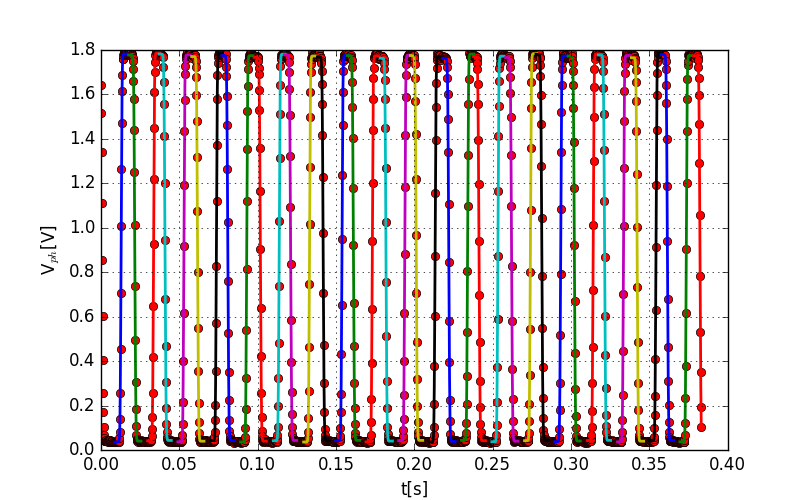
\includegraphics[width=\textwidth]{fig/perfilador/spim_foco}
        \caption{Conjunto de datos obtenidos en una petición del software de adquisición, con los ajustes efectuados}
        \label{fig:perfilador/spim_foco}
    \end{subfigure}
    \begin{subfigure}[b]{.5\textwidth}
        \centering
        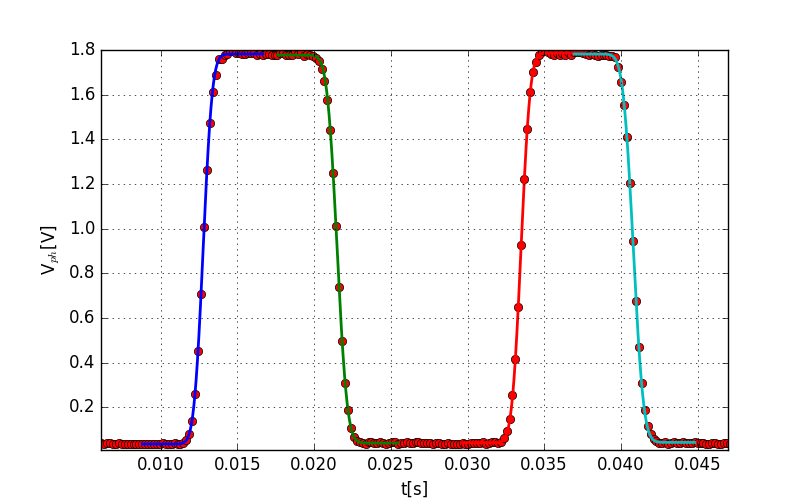
\includegraphics[width=\textwidth]{fig/perfilador/spim_foco_zoom}
        \caption{Zoom sobre la figura \ref{fig:perfilador/spim_foco} para observar las transiciones}
        \label{fig:perfilador/spim_foco_zoom}
    \end{subfigure}
    \caption{Datos obtenidos del perfilador en el foco del colimador F280FC-A}
\end{figure}

Al promediar cada perfil se obtiene que el haz mide $(3,03\pm0,15)\,$mm. Se observa una diferencia con el valor reportado por el fabricante, de 3,3$\,$mm, que se asocia a un error sistemático en la medición; puede ser por el fotodiodo utilizado, pero no se ha podido diferenciar. 

Para aseverar esta discrepancia, se hicieron mediciones manuales del perfil, que se ven en la figura \ref{fig:perfilador/spim_foco_manual}, donde queda en evidencia una discrepancia, pero con el error los datos se solapan. Resta entender la discrepancia encontrada con el valor nominal expresado por el fabricante, ya que el tamaño del haz a la salida del colimador es un parámetro determinante del tamaño (y por ende de la precisión) del lightsheet del SPIM.

\begin{figure}[H]
    \centering
    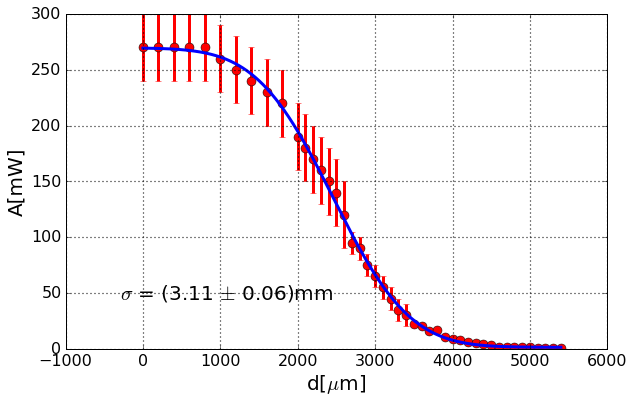
\includegraphics[width=0.6\textwidth]{fig/perfilador/calibracion_f280}
    \caption{Medición manual del perfil del haz para el colimador F280FC, con el ajuste de la función error}
    \label{fig:perfilador/spim_foco_manual}
\end{figure}

La ventaja del perfilador automático sobre la medición manual es la capacidad de realizar 40 mediciones en 0,4$\,$s como se ve en la figura \ref{fig:perfilador/spim_foco}, frente a una medición cada cinco minutos que puede lograr con un método manual, además de ser un sistema más simple de colocar y utilizar; depende del setup, puede llevar entre 10 a 15 minutos construir el perfilador manual y montarlo, mientras el perfilador automático en un par de minutos ya está midiendo. 

Para concluir las mediciones del perfilador, se midió el haz dentro del telescopio del SPIM, para observar la divergencia del haz. Estas mediciones está plasmadas en la figura \ref{fig:perfilador/spim_telescopio}, con los valores ajustados ya promediados (ya que se tienen dos tamaños de haces bien definidos) en la tabla \ref{tbl:perfilador/spim_telescopio}.

\begin{minipage}[c]{0.55\textwidth}
\begin{figure}[H]
    \centering
    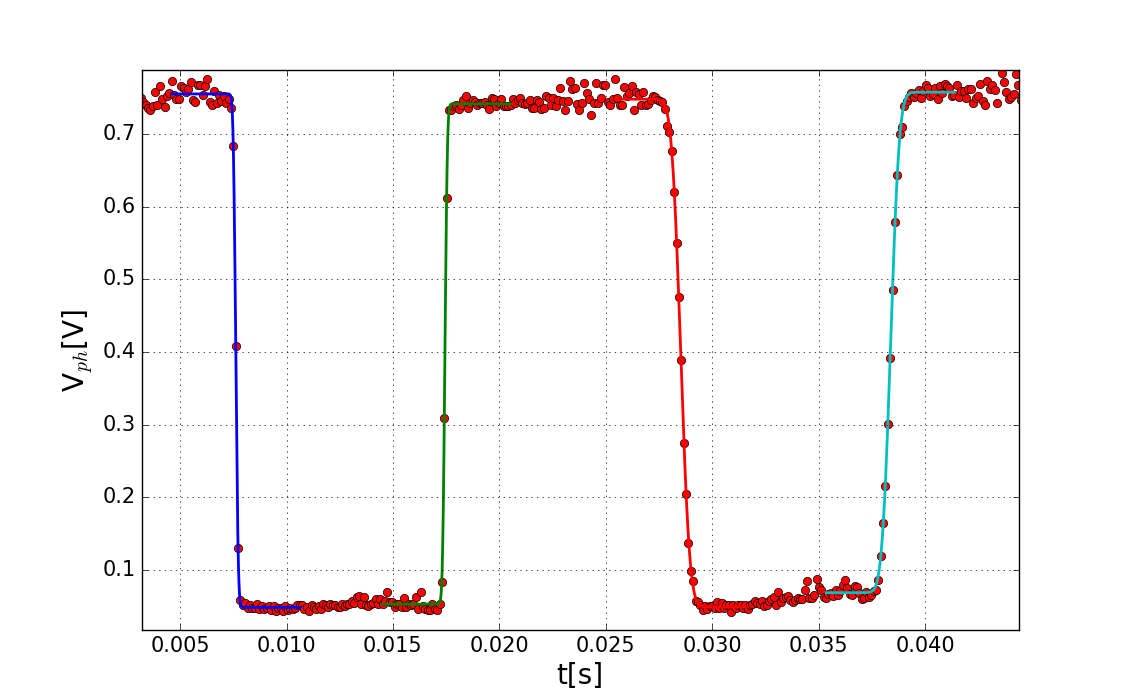
\includegraphics[width=\textwidth]{fig/perfilador/spim_telescopio}
    \caption{Datos medidos dentro del telescopio del SPIM, con las transiciones separadas y ajustadas}
    \label{fig:perfilador/spim_telescopio}
\end{figure}
\end{minipage}
%
\begin{minipage}[c]{0.35\textwidth}
    \begin{table}[H]
        \centering
        \begin{tabular}{c|c}
            Perfil & $\sigma[\text{mm}]$ \\ \hline
            1 & 0, 55$\pm$0,02  \\
            2 & 2,11$\pm$0,05 \\
        \end{tabular}
        \caption{Ajustes efectuados y promediados en la figura \ref{fig:perfilador/spim_telescopio}. Acá queda en evidencia la existencia de una divergencia del haz apreciable, considerando que entre obturaciones se observa el mismo perfil, no así entre desobturaciones}
        \label{tbl:perfilador/spim_telescopio}
    \end{table}
\end{minipage}
\\ \\

Al tener el mismo tamaño de haz entre dos obturaciones del tambor, cuando la señal es nula, pero no así entre desobturaciones, cuando la señal es máxima, se puede concluir que el perfilador está midiendo una divergencia del haz (recordar la figura \ref{fig:perfilador/corte_tambor} para tener noción de la perfilación).

Si este conjunto de mediciones lo ingresamos en la ecuación \ref{eq:perfilacion/gauss_divergence} podemos obtener la posición del foco y el ancho de cintura del haz en ese punto. De esta cuenta se obtiene dos soluciones, condensadas en la tabla \ref{tbl:perfilador/spim_telescopio_predicciones}.

\begin{table}[H]
        \centering
        \begin{tabular}{c|c|c}
            Solución & $z_0[\text{mm}]$ & $w_0[\text{mm}$] \\ \hline
            1 &  16,15 &  1,550$\times10^{-3}$  \\
            2 &  26,24 &  2,518$\times10^{-3}$\\
        \end{tabular}
        \caption{Prediciones de sobre el haz gaussiano a partir de los datos vistos en la figura \ref{fig:perfilador/spim_telescopio} y la ecuación \ref{eq:perfilacion/gauss_divergence}}
        \label{tbl:perfilador/spim_telescopio_predicciones}
\end{table}

Estas predicciones con consistentes con una perfilación con el foco dentro del tambor y con una perfilación con el foco fuera del tambor con el haz convergiendo. Ambas soluciones se explican conociendo el funcionamiento del telescopio para haces gaussianos, por lo que las mediciones  

Es preciso recordar que esta medición se hizo solo en un punto del espacio, y con ello se pudo observar la divergencia del haz. Si el camino óptico es ordenes de magnitud más grande que el tamaño del tambor, se deben hacer mediciones a varias distancias para poder observar de forma cabal la divergencia. En el caso observado, con una medición más eliminaría la ambigüedad de la medición, o conociendo de forma precisa los planos de perfilación en los datos adquiridos.

\subsection{Mediciones del polarimetro}

Las mediciones con el polarimetro fueron determinadas por la inicial calibración del material polarizante, en este caso una lámina polarizadora plástica, y luego por mediciones antes y después de la fibra del SPIM. Estas mediciones, como ya mencionamos, buscan determinar si la fibra óptica es capaz de mantener la polarización del haz incidente.

Para medir correctamente con el polarimetro, se tiene que conocer la matriz de transición de la lámina polarizadora, ya que representa la transmitancia de cada componente. Para esto, se crearon dos polarizadores rotantes con el material del polarizador y se midió la intensidad de un haz polarizado, proveniente de un láser HeNE Melles Griot 05-LGP-193, atravezando un conjunto de estados de alineación. Estas mediciones están condensadas en la tabla \ref{tbl:polarimetro/calibracion}


\begin{table}[H]
    \centering
    \begin{tabular}{c|c}
        Alineación  & P[$\mu$W] \\ \hline
        Sin láminas & 715 $\pm$ 5  \\
        Intensidad máxima, 1 lámina  & 330 $\pm$ 10 \\
        Intensidad mínima, 1 lámina  & 1,5 $\pm$ 0,1 \\
        Intensidad máxima, 2 láminas, una alineada & 160 $\pm$ 5 \\
        Intensidad minima, 2 láminas, una alineada & 0,7 $\pm$ 0,1 \\
    \end{tabular}
    \caption{Mediciones de calibración de lámina polarizadora}
    \label{tbl:polarimetro/calibracion}
\end{table}

De estas mediciones se deducen que la matriz de transferencia tiene la siguiente forma
\begin{equation}
    \begin{pmatrix} 0.461 & 0 \\ 0 & 2,097\times10^{-3} \end{pmatrix}.
\end{equation}

En esta matriz están condesados algunos detalles del polarizador. La transferencia en el eje principal es de 46,1\%, lo que representa una perdida importante de potencia luminica, y la transferencia en el eje perpendicular no es exactamente cero, lo que implica que un haz polarizado lineal generará una señal coseno cuadrado más un offset. Esta señal puede eliminarse si se conoce la intensidad del haz al llegar al polarizador. 

Esta imperfección del polarizador genera problemas solo si se trata de dicernir una polarización lineal de una eliptica, pero las demás polarizaciones quedan bien definidas. De esta forma, se hicieron mediciones con la lámina ya que nos permite separar una polarización aleatoria de una polarización definida.

Finalmente se midió la polarización antes de la fibra del SPIM, y después del colimador del SPIM, para un láser con $\lambda = 473\,$nm (de color azul) modelo DHOM-M-473-150mW (que corresponde al utilizado usualmente en el SPIM). Las mediciones está condensadas en las figuras \ref{fig:polarimetro/polarizacion_laser} y \ref{fig:polarimetro/polarizacion_fibra}, donde se recortó la medición a 1000 pasos del motor que rotaba a 10RPS, generando una ventana temporan de 0,5s. La cantidad total de datos fueron 4000, lo que son 2s de medición.

\begin{figure}[H]
    \begin{subfigure}[b]{0.5\textwidth}
        \centering
        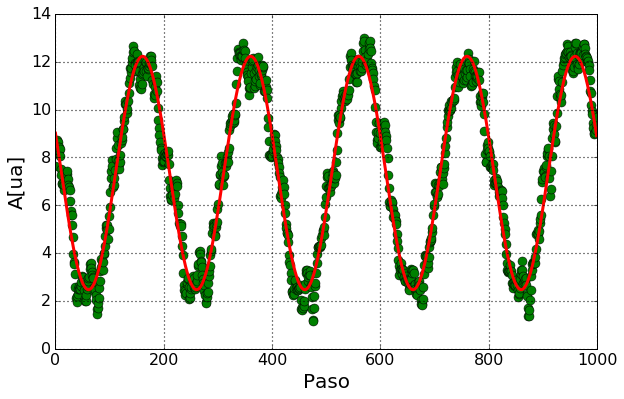
\includegraphics[width=0.8\textwidth]{fig/polarimetro/polarizacion_laser}
        \caption{Antes de la fibra óptica}
        \label{fig:polarimetro/polarizacion_laser}
    \end{subfigure}
    \begin{subfigure}[b]{0.5\textwidth}
        \centering
        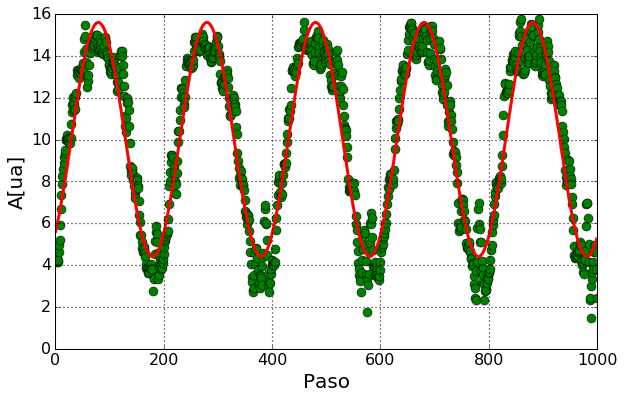
\includegraphics[width=0.8\textwidth]{fig/polarimetro/polarizacion_fibra}
        \caption{Después de la fibra óptica}
        \label{fig:polarimetro/polarizacion_fibra}
    \end{subfigure}
    \caption{Mediciones del polarimetro antes y después de la fibra óptica del SPIM para el láser azul}
\end{figure}

Al no poder controlar la intensidad del haz a la entrada de la fibra se debió intercalar filtros neutros en el camino del haz y amplificar la señal del fotodiodo. Esto conlleva a la presencia de ruido en la señal del fotodiodo, que es amplificada. 

La disposición de filtros neutros se mantuvo constante en todas las mediciones, así no se generaba diferencias de potencias que generen diferencias en el coeficiente $\alpha$. 

Al poder efectuar el ajuste correctamente en el conjunto de datos, en este caso de 4000 puntos, se puede descartar que la polarización cambie el intervalos de tiempo menores a 2s. Este ajuste a su vez descarta la polarización aleatoria, por lo que permitiría al microscopio hacer análisis de anisotropía (intercalando en el riel a la salida del colimador láminas retardadoras).

Para completar el análisis, se calculan los coeficientes $\alpha$, con la formula \ref{eq:polarizacion/alpha}. Si al atravezar la fibra se mantiene el coeficiente se mantiene, la fibra no altera la polarización a menos de una rotación de los ejes. Estos coeficientes se calculan a partir de el ajuste efectuado. 

Antes de la fibra el coeficiente obtiene un valor $\alpha = (0,664\pm 0,025)$ y después de la fibra $\alpha = (0,660\pm0,029)$. Esto determina que la fibra mantiene, dentro del error, la polarización para el laser azul, que es eliptica.

Se hicieron las mismas mediciones para los otros láseres del setup, uno verde ($\lambda = 532$nm) modelo Coherent 315M-100 y un laser rojo helio neón Melles Griot 25-LHP-151-230 (ya usado previamente), y estas mediciones está condensadas en la tabla \ref{tbl:polarimetro/mediciones}

\begin{table}[H]
    \centering
    \begin{tabular}{c|c|c}
        Laser  & $\alpha_{\text{laser}}$ & $\alpha_{\text{fibra}}$ \\ \hline
        Azul   & 0,664$\pm$0,025   & 0,660$\pm$0,029   \\
        Verde  & 0,571$\pm$0.086   & 0.539$\pm$0,064   \\
        Rojo   & 0,8916$\pm$0,0027 & 0,3482$\pm$0,0014 \\
    \end{tabular}
    \caption{Mediciones del polarimetro en el setup del SPIM para diferentes haces, antes y después de la fibra óptica}
    \label{tbl:polarimetro/mediciones}
\end{table}

Se observa que para el laser verde y azul la polarización se mantiene, dentro del error, pero no es el caso para el laser rojo. No es posible descartar un error propio de la lámina polarizadora, por lo que sería conveniente recurrir a un polarizador más cercano al ideal y repetir estas mediciones.

